\documentclass[12pt,a4paper]{ctexart}
\usepackage{geometry}
\usepackage{graphicx}
\usepackage{booktabs}
\usepackage{tabularx}
\usepackage{float}
\usepackage{xcolor}
\usepackage{hyperref}
\usepackage{enumitem}
\usepackage{fancyhdr}
\usepackage{amsmath}
\geometry{top=2.5cm,bottom=2.4cm,left=2.7cm,right=2.7cm}
\definecolor{LabGreen}{HTML}{174B36}
\definecolor{LabSoft}{HTML}{EEF5EE}
\hypersetup{colorlinks=true,linkcolor=LabGreen,urlcolor=LabGreen}
\pagestyle{fancy}
\fancyhf{}
\fancyhead[L]{LabScribe Agent}
\fancyhead[R]{软件体系结构课程设计}
\fancyfoot[C]{\thepage}
\setlength{\parindent}{2em}
\setlength{\parskip}{0.35em}
\setlist{nosep,leftmargin=2.5em}
\begin{document}
\begin{titlepage}
\centering
\vspace*{2.2cm}
{\Large\bfseries 软件体系结构课程大作业\par}
\vspace{2.2cm}
{\color{LabGreen}\Huge\bfseries LabScribe Agent\par}
\vspace{0.6cm}
{\LARGE 实验报告编写助手\par}
\vspace{0.4cm}
{\LARGE 体系结构设计文档\par}
\vfill
\renewcommand{\arraystretch}{1.8}
\begin{tabular}{rl}
姓名：& \underline{\hspace{6cm}}\\
学号：& \underline{\hspace{6cm}}\\
日期：& 2026 年 6 月\\
\end{tabular}
\vspace{2cm}
\end{titlepage}
\tableofcontents
\clearpage

\begin{quote}\small 课程：软件体系结构　　姓名：\_\_\_\_\_\_\_\_　　学号：\_\_\_\_\_\_\_\_　　日期：2026 年 6 月\end{quote}
\section{摘要}
高校实验报告往往同时依赖实验指导书、代码、运行日志、数据表、截图和指定模板。传统通用聊天模型无法稳定追踪材料来源，也难以保持 LaTeX 模板与图片位置的一致。本文设计并实现 LabScribe Agent：一个基于三层 B/S 体系结构的实验报告编写智能体。系统以 FastAPI 提供业务接口，以原生 Web 页面提供 ChatGPT 风格交互，以 SQLite 和工作区文件系统保存数据；通过 Ollama 生成向量、轻量向量检索完成 RAG，通过百度云 OCR 理解多张截图，通过 DeepSeek V4-Pro 思考模式进行问答和结构化报告规划，并输出包含图片引用的 LaTeX 源码。

系统的关键设计目标是“材料有依据、能力可替换、Demo 可运行”。外部能力均封装在适配器中；Ollama 不可用时可回退到本地哈希嵌入，因此材料仍可建立索引。系统不会把 OCR 或模型连接失败伪装成成功结果，而是在前端显示可诊断错误。

\textbf{关键词：} 软件体系结构；智能体；RAG；OCR；三层 B/S；4+1 视图

\section{项目背景与用户需求}
\subsection{应用场景与目标用户}
目标用户是需要完成课程实验、课程设计或科研实验记录的高校学生。用户通常拥有一份实验指导书、一份教师提供的报告模板、若干运行截图和零散结果数据。系统帮助用户把这些异构材料组织为结构规范、可继续编辑的实验报告，但不替代用户核验实验数据。

\subsection{角色与利益相关者}
\begin{table}[H]
\centering\small
\begin{tabularx}{\textwidth}{|X|X|}
\hline
\textbf{角色} & \textbf{关注点} \\ \hline
学生用户 & 上传方便、回答有依据、报告格式正确、图片位置合理 \\ \hline
教师/助教 & 报告结构规范、数据不被虚构、过程可演示 \\ \hline
开发维护者 & 模块低耦合、外部 API 可替换、易调试和扩展 \\ \hline
系统管理员 & 本地部署简单、依赖数量可控、敏感配置可管理 \\ \hline
\end{tabularx}
\end{table}
\subsection{功能性需求}
\begin{table}[H]
\centering\small
\begin{tabularx}{\textwidth}{|X|X|X|}
\hline
\textbf{编号} & \textbf{需求} & \textbf{验收标准} \\ \hline
FR-01 & 实验项目管理 & 可新建并切换项目，项目之间材料隔离 \\ \hline
FR-02 & 多格式材料读取 & 支持 DOCX、LaTeX、PDF、TXT、Markdown 等文本提取 \\ \hline
FR-03 & 模板读取 & 可将 TEX 标记为模板，输出时应用模板结构 \\ \hline
FR-04 & 多图片 OCR & 一次上传多张图片，调用百度 SDK 提取中英文文字 \\ \hline
FR-05 & RAG 索引与问答 & 文档切块、向量化、相似度检索，回答附材料来源 \\ \hline
FR-06 & 报告智能生成 & DeepSeek V4-Pro 基于检索材料与模板章节生成结构化报告，不虚构数据 \\ \hline
FR-07 & 图片插入 & LaTeX 生成 figure 引用和配套图片目录 \\ \hline
FR-08 & LaTeX 导出 & 可下载 TEX 文件，并保留可编辑源代码 \\ \hline
FR-09 & 历史记录 & 保存对话和已生成报告，刷新页面后仍可查看 \\ \hline
FR-10 & 服务状态提示 & 显示 DeepSeek/OCR 配置与 Ollama 在线状态 \\ \hline
\end{tabularx}
\end{table}
\subsection{核心交互流程}
\begin{enumerate}
\item 用户新建实验项目。
\item 用户上传实验材料、多张截图和可选模板。
\item 系统解析文档；图片先经 OCR，文字与文档内容一起切块并嵌入向量库。
\item 用户可通过对话提出问题。系统检索相关片段，DeepSeek 严格依据片段回答并返回引用。
\item 用户填写写作要求、图片安排和高级提示词。报告智能体检索上下文、提取模板章节，并让 V4-Pro 生成包含章节和图片归属的 JSON 计划。
\item 导出器把中间稿映射为 LaTeX 章节与 figure，保存并提供下载。
\end{enumerate}
\subsection{非功能性需求}
\begin{itemize}
\item \textbf{易用性：} 单页式工作区，主要任务不超过三次操作；错误使用中文描述。
\item \textbf{响应性：} 本地项目查询在 500 ms 内完成；耗时 AI 调用给出加载状态。
\item \textbf{可扩展性：} LLM、嵌入、OCR、存储和导出均通过独立服务类隔离。
\item \textbf{可靠性：} 上传文件使用项目独立目录；输出历史持久化；外部服务故障可诊断。
\item \textbf{可维护性：} 表示层、业务层、数据层只沿规定方向依赖；业务服务单一职责。
\item \textbf{安全性：} 文件名去除目录成分，限制单文件大小；\texttt{.env} 不纳入版本控制；发布代码前应轮换课程 Demo 密钥。
\item \textbf{可移植性：} Windows/macOS/Linux 均可用 Conda 创建环境；本地只依赖 Python 与可选 Ollama。
\end{itemize}
\section{功能分解}
\subsection{顶层功能模块}
\begin{quote}\small 本结构图的可渲染 Mermaid 源码见配套 Markdown 文档。\end{quote}
\subsection{模块职责与接口}
\begin{table}[H]
\centering\small
\begin{tabularx}{\textwidth}{|X|X|X|}
\hline
\textbf{模块} & \textbf{核心职责} & \textbf{输入/输出} \\ \hline
API Routes & 参数校验、HTTP 状态映射、调用业务服务 & JSON/Multipart → JSON/File \\ \hline
DocumentService & 解析文档并归一化文本 & Path → Text \\ \hline
OCRService & 使用课程提供的 BaiduAi SDK 识图 & Image → OCR Text \\ \hline
EmbeddingService & 调用 Ollama；故障时确定性降级 & Text[] → Vector[] \\ \hline
RAGService & 分块、写入向量、Top-K 检索 & Query → Relevant Chunks \\ \hline
DeepSeekService & V4-Pro 思考模式、JSON 输出、超时和错误转换 & Messages → Structured Completion \\ \hline
ReportAgent & 感知、检索、决策、执行的业务编排 & Project → ReportRecord \\ \hline
ReportService & 中间 Markdown 转 LaTeX & Markdown + Images → TEX + Assets \\ \hline
SQLiteRepository & 项目、资源、向量、消息、报告持久化 & Domain Object ↔ SQLite \\ \hline
\end{tabularx}
\end{table}
\subsection{依赖约束}
表示层只通过 HTTP 使用 API；API 不直接写 SQL，而调用业务服务和仓储；业务服务可依赖抽象意义上的仓储和外部适配器；数据层不知道前端和 HTTP 的存在。\texttt{ReportAgent} 负责流程编排，但不负责文档解析、网络协议或文件排版，以避免形成“上帝类”。

\section{软件体系结构风格设计}
\subsection{三层 B/S 风格}
系统采用三层 B/S 作为总体风格：浏览器中的表示层、FastAPI 业务逻辑层、SQLite/文件系统数据层。该风格与本地 Web Demo 匹配，浏览器零安装，后端集中复用 AI 能力，数据访问也能统一管理。

\begin{quote}\small 本结构图的可渲染 Mermaid 源码见配套 Markdown 文档。\end{quote}
\textbf{优点：} 职责清晰、易测试、易替换前端或数据库；部署简单；API 也能被未来移动端复用。\textbf{缺点：} 小型项目类和接口数量有所增加；同步生成报告时业务进程会等待外部 API。后续可引入任务队列缓解长任务问题。

\subsection{仓储（Repository）风格}
系统把 SQLite 作为共享仓储，项目元数据、文档块向量、对话和报告记录由统一仓储访问。对当前小项目而言，它免运维、事务完整、备份简单，优于部署独立向量数据库。向量以 JSON 存储并在内存计算余弦相似度；规模达到数十万块后，可在不改变业务 API 的情况下替换为 Chroma、FAISS 或 pgvector。

\subsection{管道—过滤器风格}
材料处理体现管道—过滤器：\texttt{上传 → 类型判断 → 文档解析/OCR → 文本归一化 → 切块 → 嵌入 → 持久化}。每个过滤器处理一种转换，便于独立测试和替换。报告生成则为 \texttt{检索 → 提示装配 → LLM 草拟 → 图片占位解析 → 格式导出}。

\subsection{风格适配性总结}
三层风格解决系统静态职责划分，仓储风格解决数据一致性，管道—过滤器解决材料处理和报告生成流程。三者并非互斥：它们分别作用于系统层次、数据协作和处理过程，组合后既适合课程 Demo，也保留真实演进路径。

\section{智能体设计模式分析}
\subsection{RAG（检索增强生成）模式}
\textbf{问题：} 大模型不知道用户私有实验材料，直接让模型写报告容易产生幻觉。\textbf{方案：} 智能体先将材料向量化；问答或生成前，根据任务检索 Top-K 片段，把片段及来源加入提示。\textbf{系统应用：} \texttt{RAGService.search} 以余弦相似度返回材料片段，问答结果显示文件名、相似度和摘要。报告生成检索较多片段，覆盖目标、步骤、数据与 OCR 结果。

该模式改善事实可追溯性并降低上下文长度。局限是检索质量受分块与嵌入模型影响；因此系统保留来源信息，并要求模型在证据不足时明确说明。

\subsection{Tool Use（工具使用）模式}
\textbf{问题：} 单个模型既不能直接可靠读取二进制 Word 材料，也不应自行模拟 OCR 或文档排版。\textbf{方案：} 把能力封装为确定性工具，由编排器选择和组合。\textbf{系统工具：} 文档解析器、百度 OCR、Ollama 嵌入、SQLite 检索和 LaTeX 导出器。模型负责语言推理，工具负责可验证的输入输出操作。

工具模式降低模型负担，并使外部服务可替换。例如百度 OCR 可以替换为 PaddleOCR，业务流程不必重写。

\subsection{Planner–Executor（计划—执行）模式}
报告生成不是一次随意对话，而是有明确阶段的目标任务。\texttt{ReportAgent} 充当 Planner：提取模板顶层章节，把每张图片绑定到稳定 ID、原文件名、尺寸和 OCR 文本，要求 V4-Pro 返回经过 JSON Schema 校验的章节与图片归属计划。\texttt{ReportService} 作为 Executor，整体替换模板示例正文，确定性生成段落、标题、ASCII 图片路径、\texttt{figure} 与文件。计划与执行分离后，模型不能直接写磁盘，也不能产生任意路径；漏分配的图片会被系统补入结果或截图章节。

\subsection{Guardrails（护栏）模式}
系统提示明确要求“不虚构实验数据、信息不足时说明”；API 对文件大小、项目存在性和输出格式进行校验；文件名经 \texttt{Path.name} 去除目录穿越；外部服务错误转为可见的 502 信息。这些护栏共同约束智能体的输入、推理和执行边界。

\section{4+1 视图分析}
按照课程课件，逻辑视图服务最终用户的功能需求；开发视图表现模块组织；进程视图关注并发、通信和运行特性；物理视图描述软件到硬件节点的映射；场景视图以关键用例把四种视图串联。

\subsection{逻辑视图（类/组件图）}
\begin{figure}[H]
\centering
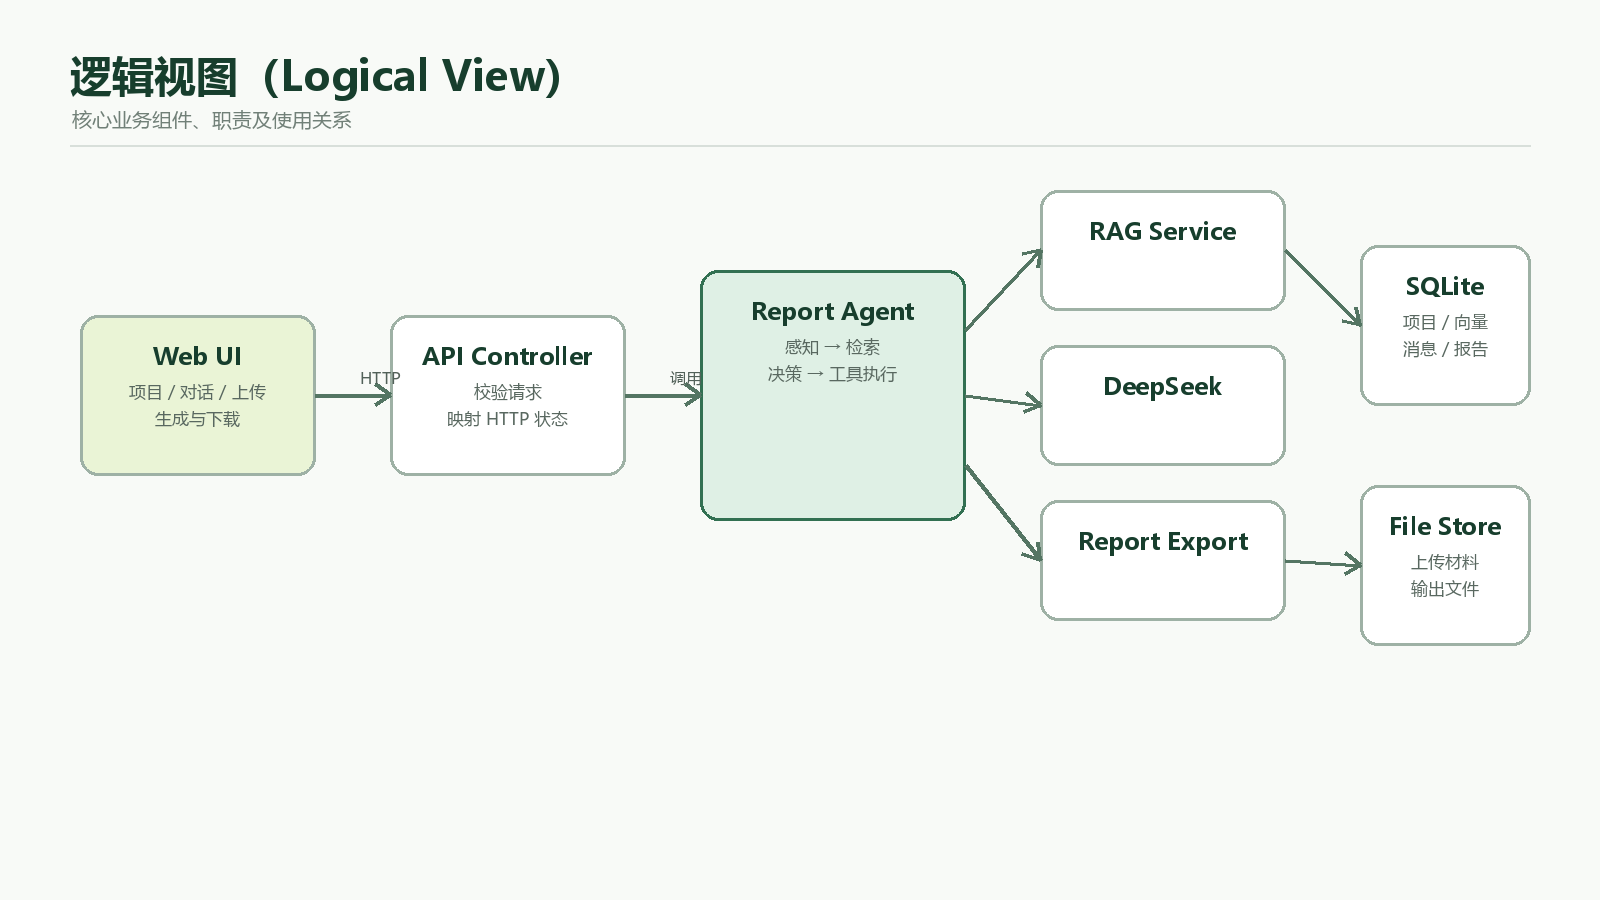
\includegraphics[width=\textwidth]{diagrams/01_逻辑视图.png}
\caption{逻辑视图（类/组件图）}
\end{figure}
该视图保持单一、内聚的领域对象模型。\texttt{Project} 聚合资源、消息和报告；服务以组合方式协作，不通过继承耦合外部厂商。

\subsection{开发视图（包/组件图）}
\begin{figure}[H]
\centering
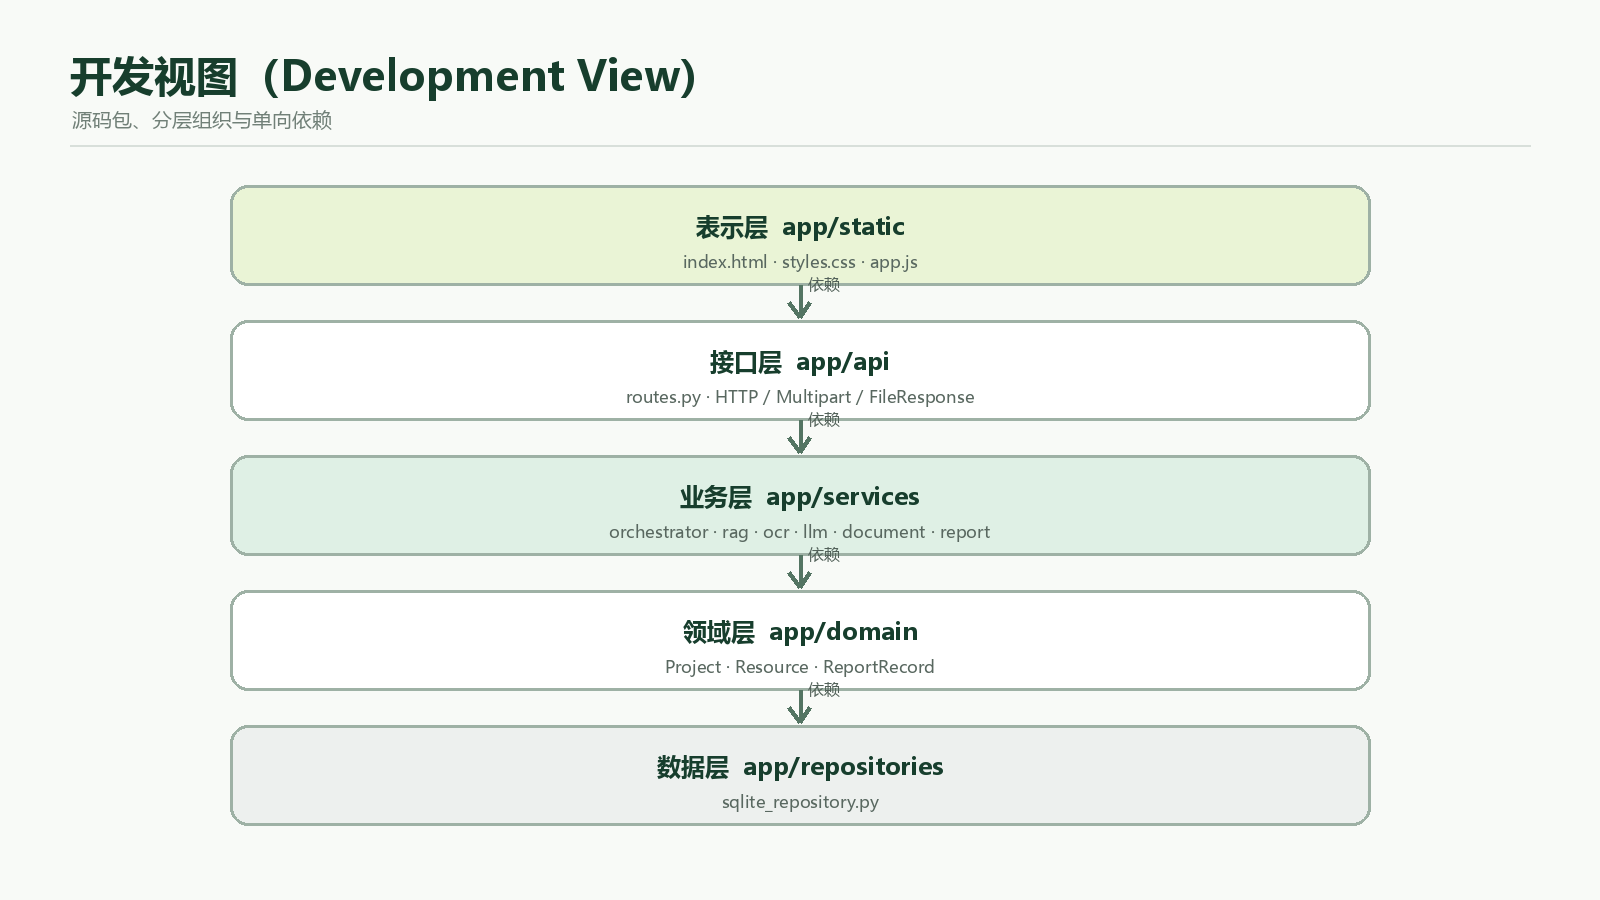
\includegraphics[width=\textwidth]{diagrams/02_开发视图.png}
\caption{开发视图（包/组件图）}
\end{figure}
目录层次遵循“高层使用低层、低层不反向依赖页面”的规则。外部 \texttt{BaiduAi/aip} 是供应商 SDK，仅被 OCR 适配器引用。

\subsection{进程视图（运行与通信）}
\begin{figure}[H]
\centering
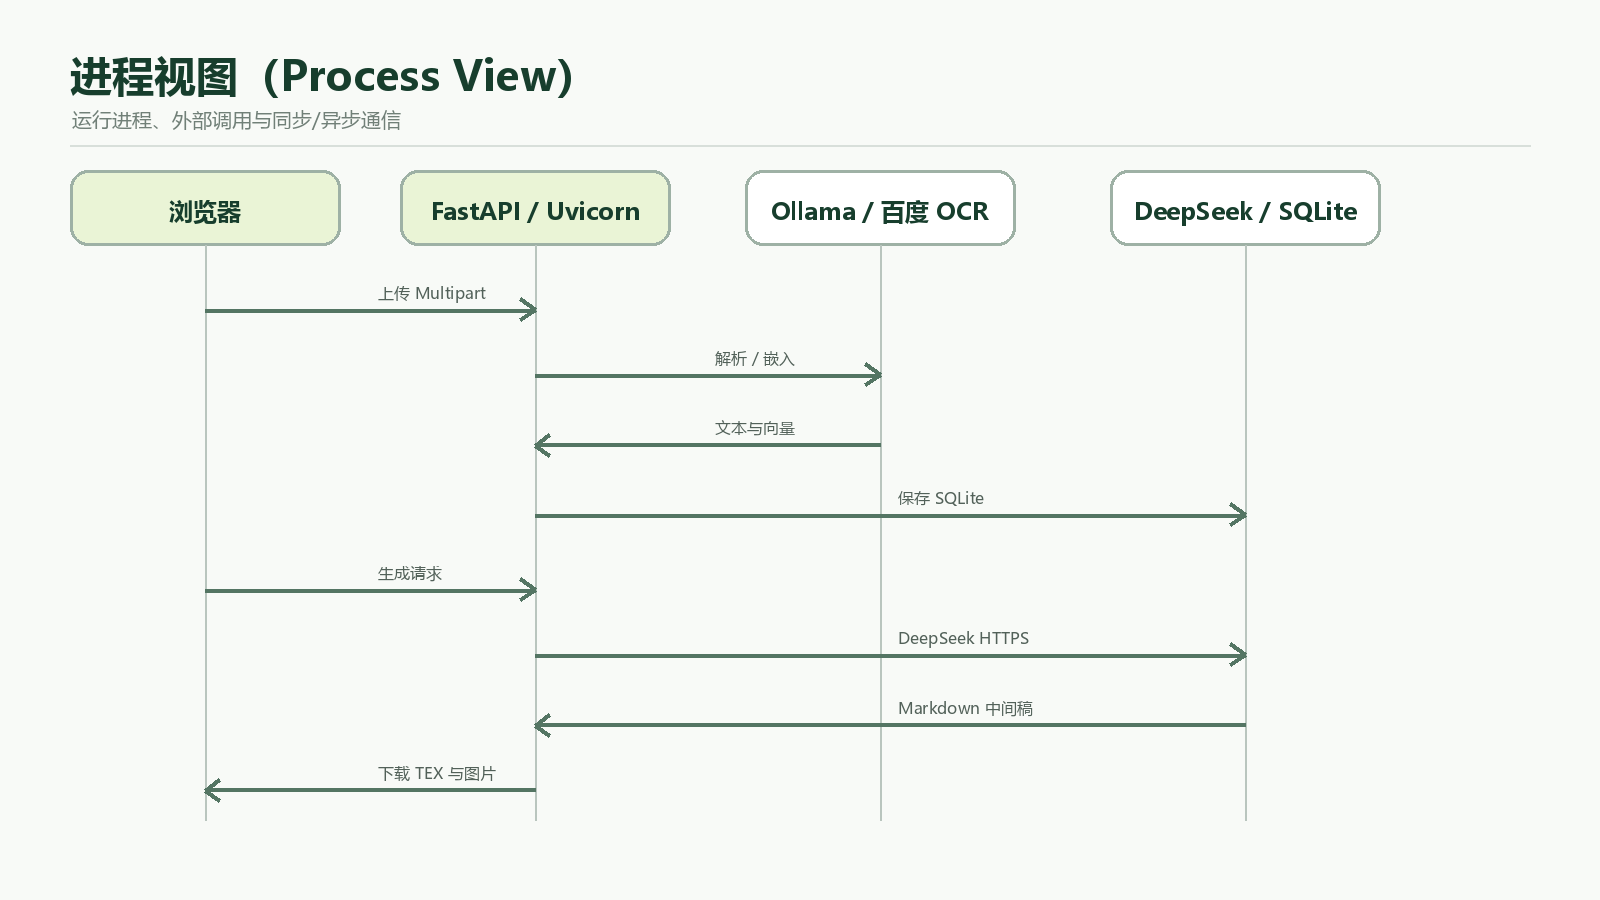
\includegraphics[width=\textwidth]{diagrams/03_进程视图.png}
\caption{进程视图（运行与通信）}
\end{figure}
当前 Demo 使用单个 Uvicorn 进程，异步 HTTP 客户端在等待 DeepSeek/Ollama 时释放事件循环。SQLite 写入是短事务。OCR SDK 是同步调用，数据量较小时可接受；生产化时应把 OCR 与生成任务放入 Celery/RQ 工作进程，前端通过任务 ID 轮询或 WebSocket 获取进度。

\subsection{物理视图（部署图）}
\begin{figure}[H]
\centering
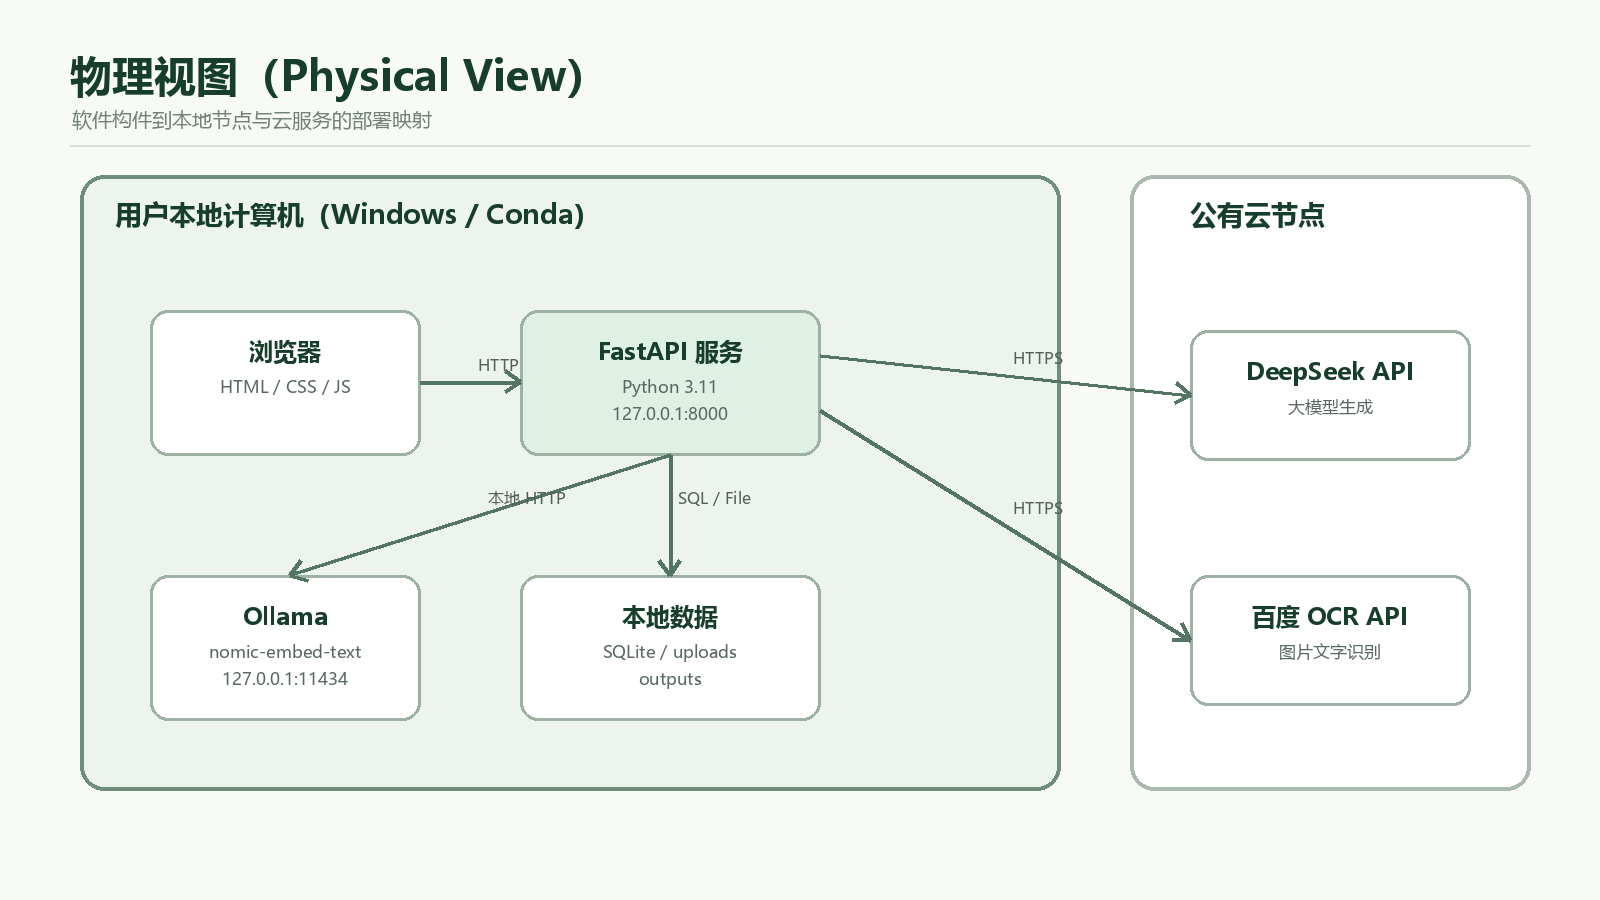
\includegraphics[width=\textwidth]{diagrams/04_物理视图.png}
\caption{物理视图（部署图）}
\end{figure}
软件主要部署在单机节点，避免服务器运维。浏览器与应用服务器逻辑分离，仍属于 B/S；AI 云服务经 HTTPS 访问。输出和数据库位于项目 \texttt{data} 目录，便于整体备份。

\subsection{场景视图（关键用例与活动图）}
\begin{figure}[H]
\centering
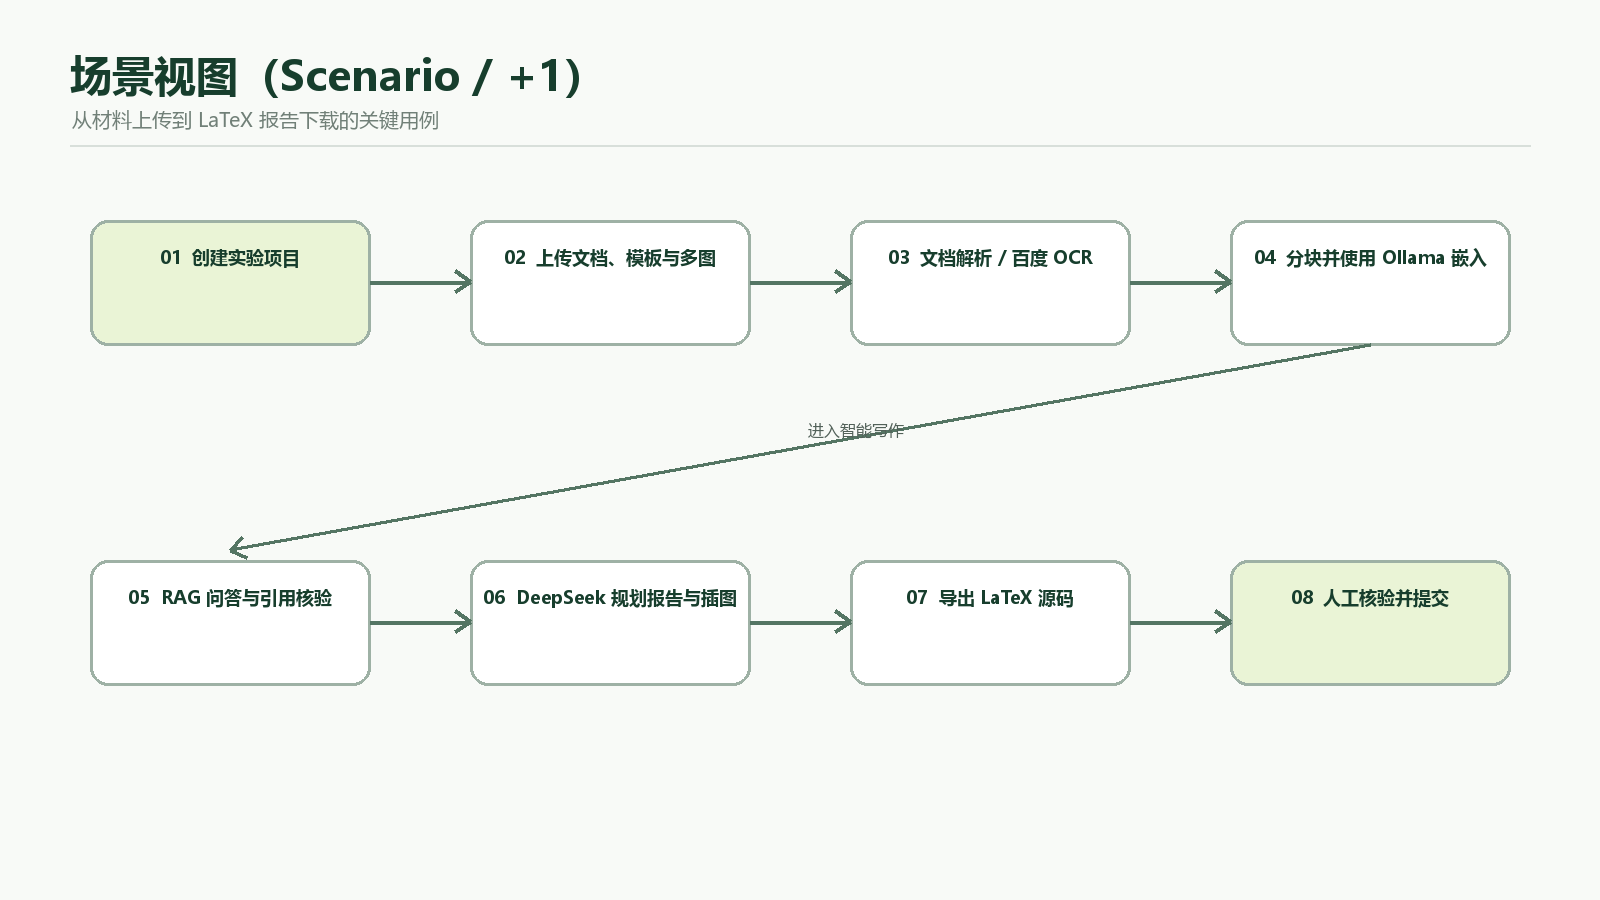
\includegraphics[width=\textwidth]{diagrams/05_场景视图.png}
\caption{场景视图（关键用例与活动图）}
\end{figure}
这一场景覆盖逻辑视图的核心服务、开发视图的主要模块、进程视图中的外部调用，以及物理视图的浏览器—本地服务—云 API 通信，是 Demo 视频的主线。

\section{数据与接口设计}
\subsection{数据模型}
\begin{table}[H]
\centering\small
\begin{tabularx}{\textwidth}{|X|X|X|}
\hline
\textbf{表} & \textbf{关键字段} & \textbf{说明} \\ \hline
projects & id, title, description, created\_at & 实验项目 \\ \hline
resources & project\_id, kind, path, extracted\_text, error & 材料、模板和图片 \\ \hline
chunks & resource\_id, content, embedding & RAG 文本块及 JSON 向量 \\ \hline
messages & project\_id, role, content & 对话历史 \\ \hline
reports & project\_id, format, path & 输出记录 \\ \hline
\end{tabularx}
\end{table}
所有主键使用 UUID 或自增整数。文件不写入数据库 BLOB，只保存项目隔离后的路径，避免数据库膨胀。

\subsection{REST API}
API 使用 Pydantic 校验 JSON，上传采用 Multipart，下载使用流式文件响应。典型接口包括：\texttt{POST /api/projects}、\texttt{POST /api/projects/\{id\}/resources}、\texttt{POST /api/projects/\{id\}/chat}、\texttt{POST /api/projects/\{id\}/reports} 和 \texttt{GET /api/reports/\{id\}/download}。FastAPI 自动生成 \texttt{/docs} OpenAPI 页面，便于接口演示与测试。

\subsection{RAG 算法}
文本按约 700 字符切块，并保留 100 字符重叠；优先在换行或句号处截断。Ollama 默认模型为 \texttt{nomic-embed-text}。检索阶段对查询向量与同项目全部块计算余弦相似度：

\[similarity(q,d)=\frac{q\cdot d}{\lVert q\rVert\lVert d\rVert}\]
当前实现适合课程规模。若每项目约 100 份材料、每份 50 块，总计 5,000 向量，内存扫描足以完成交互；规模增长时替换数据层即可。

\section{关键实现说明}
\subsection{图片理解与插图}
图片上传后保存原文件，调用课程提供的 \texttt{BaiduAi/aip} SDK 的通用文字识别接口。OCR 文本既进入 RAG，也与图片 ID、原文件名和像素尺寸组成图片清单。V4-Pro 为每个图片 ID 选择目标章节和证据型图注；导出器验证 ID 不重复，把图片复制到纯 ASCII 资源目录，并生成 XeLaTeX 可用的 \texttt{figure}、\texttt{includegraphics}、题注和原文件名注释。DeepSeek API 本身不接收图片二进制，因此视觉文字内容由百度 OCR 提供，路径与插入动作由本地工具完成。

\subsection{模板策略}
LaTeX 模板优先替换 \texttt{\{\{TITLE\}\}} 与 \texttt{\{\{REPORT\_CONTENT\}\}}；若模板没有占位符，则在 \texttt{\textbackslash{}end\{document\}} 前插入正文。无模板时生成可由 XeLaTeX 编译的 \texttt{ctexart} 源码，但系统按作业范围不负责 LaTeX 编译。Word 文件仅作为可读取的实验材料，不作为输出格式。

\subsection{异常与降级}
\begin{itemize}
\item Ollama 不在线：使用 256 维本地哈希嵌入，保证 Demo 流程可继续，并在状态栏标记“离线降级”。
\item 百度 OCR 失败：资源仍保存，错误显示在材料列表；不伪造图片文字。
\item DeepSeek 失败：API 返回 502 和可读错误；不生成空报告文件。
\item 不支持的文件：保留资源和错误说明，其他已上传文件继续处理。
\item 文件过大：超过 30 MB 立即删除不完整文件并返回 413。
\end{itemize}
\section{测试与验证}
\subsection{测试策略}
\begin{table}[H]
\centering\small
\begin{tabularx}{\textwidth}{|X|X|}
\hline
\textbf{层次} & \textbf{测试重点} \\ \hline
单元测试 & 文本分块重叠、哈希嵌入确定性、余弦排序、LaTeX 导出 \\ \hline
API 测试 & 项目创建、上传校验、无材料生成错误、下载路径 \\ \hline
集成测试 & Ollama 嵌入、百度 OCR、DeepSeek 对话与报告生成 \\ \hline
UI 验收 & 新建项目、拖拽上传、材料错误、引用展示、LaTeX 下载 \\ \hline
\end{tabularx}
\end{table}
\subsection{可追踪验收场景}
准备一份含特定实验参数的 TXT、一张包含结果文字的 PNG 和一个 LaTeX 模板。上传后询问该参数，应在回答下方看到对应文件引用；断开 Ollama 后再次问答，系统状态应显示离线降级且仍能检索；生成后应看到 \texttt{\_assets} 目录和正确的 \texttt{includegraphics} 路径。

\section{运行与演示}
\begin{verbatim}
conda env create -f environment.yml
conda activate lab-report-agent
ollama pull nomic-embed-text
python run.py
\end{verbatim}
访问 \texttt{http://127.0.0.1:8000}。演示视频建议控制在 2 分钟：20 秒介绍目标与三层架构，40 秒上传并展示 OCR/RAG，40 秒生成 LaTeX 与图片目录，20 秒展示 4+1 视图与总结。

\section{设计评价与演进方向}
本系统已覆盖智能体的“感知—决策—执行”：文档解析和 OCR 完成感知，RAG 与 DeepSeek 完成证据检索和内容决策，格式导出器完成可验证执行。三层架构让前端、业务和数据各自演进；RAG、工具使用、计划—执行和护栏模式使系统不只是一个聊天页面。

当前不足包括：SQLite 向量为线性扫描；同步 OCR 可能阻塞；LaTeX 模板只支持约定占位符或文末插入；没有账号权限与协作。下一阶段可引入后台任务队列、真正的向量索引、模板语义槽位协议、报告版本差异和人工审批环节。若部署到公网，还必须把 API 密钥移入密钥管理服务、加入登录鉴权、病毒扫描、限流和审计。

\section{结论}
LabScribe Agent 在较低部署成本下完成了异构材料读取、多图 OCR、RAG 问答、基于模板的智能写作和 LaTeX 源码导出。设计以三层 B/S 为骨架，以仓储和管道风格补充数据与处理过程，并通过完整 4+1 视图验证静态模块、运行进程、物理部署和用户场景的一致性。项目可直接用于课程 Demo，也为后续扩展为真实实验知识工作台留下了清晰接口。

\appendix
\section{个人/团队分工表（尾页）}
\begin{table}[H]
\centering\small
\begin{tabularx}{\textwidth}{|X|X|X|X|}
\hline
\textbf{姓名} & \textbf{学号} & \textbf{负责模块} & \textbf{承担权重} \\ \hline
\_\_\_\_\_\_\_\_ & \_\_\_\_\_\_\_\_ & 用户需求、体系结构、智能体模式、4+1 视图、Demo 实现、测试与文档 & 100\% \\ \hline
\end{tabularx}
\end{table}
\begin{quote}\small 单人作业贡献系数为 1；提交前请填写姓名和学号，并按“学号\_姓名\_Agent体系结构文档.pdf”命名。\end{quote}
\end{document}
